\begin{pastexam}[label={px:ntu-107-esoe-ds-06}]{臺大工科海洋所 107 學年度 第 6 題}
（問答；10 分）

\textbf{(10 \%)} Suppose we are using a tree-based disjoint set data structure with union-by-size and
path compression.
\begin{enumerate}[label=\alph*.]
\item (5 \%) Draw a 16-node disjoint set tree that has the maximum height possible. \textbf{Hint}: The
tree must be one that can be created through union and find operations.
\item (5 \%) What is the minimum number of find operations it would take to transform the tree in (a)
to have the minimum height possible? Why?
\end{enumerate}
\end{pastexam}

\begin{pastsoln}
答案：a. 下圖的樹（二項樹 $B_4$），最深的節點在根下面第 $4$ 層；b. $7$ 次。

高度有兩種算法：資結書第~13~章照第~7~章數節點（單一節點高度 $1$），很多考卷數邊（單一節點
高度 $0$）。 下面兩種都寫。 Union 照資結書虛擬碼~13.3：兩棵一樣大時，第二個參數的根接到第一個
參數的根底下。

\textbf{a.} 資結書定理~13.2：依大小合併（有沒有路徑壓縮都一樣），$s$ 個節點的樹高度不超過
$\lfloor \lg s \rfloor + 1$。 理由是節點每變深一層，它所在的樹至少變成兩倍大。 $s = 16$ 時高度
最多 $5$（數邊是 $4$）。 要達到這個上界，每次合併都要是「兩棵一樣大的樹」，而且過程中不能做會
壓縮路徑的 Find。 節點編號 $1$--$16$，依序做
\begin{center}
\begin{tabular}{ll}
\toprule
第一輪 & Union$(1, 2)$, Union$(3, 4)$, Union$(5, 6)$, \ldots, Union$(15, 16)$ \quad（$8$ 棵 $2$ 個節點的樹） \\
第二輪 & Union$(1, 3)$, Union$(5, 7)$, Union$(9, 11)$, Union$(13, 15)$ \quad（$4$ 棵 $4$ 個節點） \\
第三輪 & Union$(1, 5)$, Union$(9, 13)$ \quad（$2$ 棵 $8$ 個節點） \\
第四輪 & Union$(1, 9)$ \quad（$1$ 棵 $16$ 個節點） \\
\bottomrule
\end{tabular}
\end{center}
每次 Union 的兩個參數都是根，裡面呼叫的 Find-Set 直接回傳，沒有壓縮任何路徑。 結果：
\begin{center}
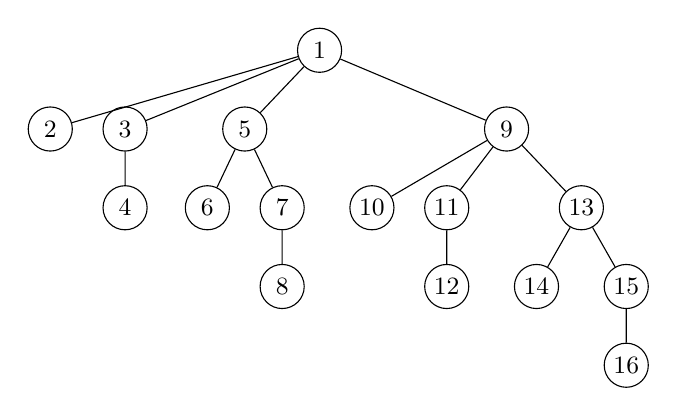
\begin{tikzpicture}[x=0.95cm,y=1.0cm,v/.style={circle,draw,inner sep=0pt,minimum size=5.6mm,font=\small}]
\node[v] (1) at (3.6,0) {1};
\node[v] (2) at (0,-1) {2};
\node[v] (3) at (1,-1) {3};
\node[v] (4) at (1,-2) {4};
\node[v] (5) at (2.6,-1) {5};
\node[v] (6) at (2.1,-2) {6};
\node[v] (7) at (3.1,-2) {7};
\node[v] (8) at (3.1,-3) {8};
\node[v] (9) at (6.1,-1) {9};
\node[v] (10) at (4.3,-2) {10};
\node[v] (11) at (5.3,-2) {11};
\node[v] (12) at (5.3,-3) {12};
\node[v] (13) at (7.1,-2) {13};
\node[v] (14) at (6.5,-3) {14};
\node[v] (15) at (7.7,-3) {15};
\node[v] (16) at (7.7,-4) {16};
\draw (1)--(2) (1)--(3) (1)--(5) (1)--(9) (3)--(4) (5)--(6) (5)--(7) (7)--(8)
  (9)--(10) (9)--(11) (9)--(13) (11)--(12) (13)--(14) (13)--(15) (15)--(16);
\end{tikzpicture}
\end{center}
路徑 $16 \to 15 \to 13 \to 9 \to 1$ 有 $4$ 條邊，高度 $5$（數邊是 $4$），達到上界，所以是高度最大
的樹。 各層的節點數是 $1, 4, 6, 4, 1$，也就是 $\binom{4}{d}$。

\textbf{b.} 只做 Find 的話，高度最小是 $2$（數邊是 $1$）：根在上面，其他 $15$ 個節點都直接接在
根下面。 $16$ 個節點不可能只有一層。

\textbf{至少要 $7$ 次。} 路徑壓縮只會把 Find 路徑上的節點改接到根，而且只有根會多出子節點。 所以：
(1) 一個節點的父節點要改變，它必須在某次 Find 的路徑上；(2) 葉節點（不是根）永遠是葉節點，它
在某次 Find 的路徑上，只可能是因為那次 Find 就是找它自己。 a 小題的樹裡，深度 $\ge 2$ 的葉節點
有 $4, 6, 10$（深度 $2$）、$8, 12, 14$（深度 $3$）、$16$（深度 $4$），共 $7$ 個；它們的父節點都
不是根，都得改，所以每一個都要被 Find 一次，至少 $7$ 次。

\textbf{$7$ 次就夠。} 做 Find$(4)$、Find$(6)$、Find$(8)$、Find$(10)$、Find$(12)$、Find$(14)$、
Find$(16)$（順序不拘）。 每一個深度 $\ge 2$ 的節點都是這 $7$ 個葉節點之一的祖先或它本身：
$3$ 是 $4$ 的、$5, 7$ 是 $8$ 的、$11$ 是 $12$ 的、$13, 15$ 是 $16$ 的祖先，深度 $1$ 的 $2, 9$ 本來就
接在根下面。 所以 $7$ 次 Find 之後，所有節點都直接接在 $1$ 下面，高度變成 $2$。 例如 Find$(16)$
一次就把 $16, 15, 13$ 都改接到 $1$（$9$ 本來就是）。
\end{pastsoln}
